% Supplemental Material of paper.tex.  Build: tectonic -X compile sm.tex
% Sources of every number are given in the captions (notebooks in ../notebooks/, which print them).
\documentclass[pre,onecolumn,superscriptaddress,nofootinbib]{revtex4-2}
\usepackage{amsmath,amssymb,bm}
\usepackage{graphicx}
\usepackage{xcolor}
\graphicspath{{figures/}}
\usepackage[hidelinks]{hyperref}

\newcommand{\E}{\mathbb E}
\newcommand{\Var}{\operatorname{Var}}
\newcommand{\Sb}{\bar S}
\newcommand{\PhiN}{\Phi_{\mathcal N}}
\newcommand{\todo}[1]{\textcolor{red}{[TODO: #1]}}
\renewcommand{\thesection}{S\arabic{section}}
\renewcommand{\theequation}{S\arabic{equation}}
\renewcommand{\thetable}{S\arabic{table}}
\renewcommand{\thefigure}{S\arabic{figure}}

\begin{document}

\title{Supplemental Material: Interaction heterogeneity and the multiscaling of firm growth volatility}
\author{Ludovico Furlanetto}
\date{\today}
\maketitle

\noindent Every number and figure below is printed or drawn by a notebook of the companion repository,
\url{https://github.com/NotLudovico/dynamical-model-for-economics}; captions name the notebook.

%======================================================================
\section{Relative sizes and the standard model}
\label{sec:relative}

Write $x_i=mS_i$ in Eq.~(2) of the main text.  By It\^o's rule, with $\bar f=\dot m/m$ the drift of the
mean firm,
\begin{equation}
dS_i=S_i\big[F_i-\bar f\big]dt+\sqrt{DS_i}\,dW_i-\frac{S_i}{N}\sum_j\sqrt{DS_j}\,dW_j+O(N^{-1})\,dt,\qquad
F_i=1-S_i+\sum_jJ_{ij}S_j ,
\label{eq:rel}
\end{equation}
and $\bar f=N^{-1}\sum_iS_iF_i$ is the value that keeps $\sum_iS_i=N$ between entries.  The third term, of order
$N^{-1/2}$, is the share of the aggregate noise that each firm carries.  Each entry adds $D$ to $\sum_iS_i$, i.e.\
$Dm$ to the economy, and multiplies every relative size by $1-D/N$; at a rate $N\nu$ of entries this is a drift
$-D\nu S_i$, so the growth rate of the mean firm is $\bar f=N^{-1}\sum_iS_iF_i+D\nu$, the value used in the field
throughout.  This is a replicator equation
with birth--death noise; with $\Phi_i=F_i+S_i-\bar f$ it is Eq.~(3).  If $\bar f$ self-averages to a constant
$f^*$ at large $N$, the substitution $S=ry$, $t'=rt$ with $r=1-f^*$ gives
\begin{equation}
dy_i=y_i\Big[1-y_i+\sum_jJ_{ij}y_j\Big]dt'+\sqrt{(D/r^2)\,y_i}\,dW_i' ,
\end{equation}
the GLV with demographic noise of Ref.~\cite{altieri2021} on the same graph, with noise $D/r^2$ and newborns
of size $D/r$.  The
stationary statistics of relative sizes are therefore those of the standard model with renormalised
noise; the normalisation adds the growth rate $f^*$ as an output, a common mode $\bar f(t)-f^*$ at
finite $N$, and observables measured relative to the mean firm.  In the deterministic version the
floor $\lambda(m-x_i)$ becomes an immigration $\lambda/r^2$ and a shift $-\lambda/r$ of the growth rate, and up to
that $O(\lambda)$ shift the model is the migration-supported GLV of Refs.~\cite{bunin2017,mallmin2024}.

%======================================================================
\section{Heterogeneous mean-field theory and the deterministic stability line}
\label{sec:hdmft}

\paragraph{Degree classes.}  Group the nodes into classes $p$ with fractions $\rho_p$ and degrees
$k_p$, and let $P_{pr}$ be the probability that a node of class $p$ links to one of class $r$, with
$k_p/N=\sum_r\rho_rP_{pr}$.  The uncorrelated choice $P_{pr}=k_pk_r/(NC)$ exceeds one for pairs of hubs
at $\alpha=2.5$; we use the soft-configuration kernel $P_{pr}=h_ph_r/(h_ph_r+C/N)$ with hidden degrees fixed
by the degree constraint \cite{patil2026}, and write $K_{pr}=N\rho_rP_{pr}/C$.

\paragraph{Effective process.}  For $C\to\infty$ the mean part of the interaction field on a node of
class $p$ tends to $\mu B_p$ and, by the dynamical cavity argument
\cite{bunin2017,galla2018,aguirrelopez}, the random part to a Gaussian process of covariance
$\sigma^2q_p(t,t')$, with
\begin{equation}
B_p(t)=\sum_rK_{pr}\E[S_r(t)],\qquad q_p(t,t')=\sum_rK_{pr}\E[S_r(t)S_r(t')] .
\label{eq:closure}
\end{equation}
At zero reciprocity there is no reaction term.  Each class obeys Eq.~(3) of the main text with field
$\Phi_p(t)=1-\bar f(t)+\mu B_p(t)+\sigma\eta_p(t)$, $\E[\eta_p(t)\eta_p(t')]=q_p(t,t')$, closed by
Eq.~\eqref{eq:closure} and by $\sum_p\rho_p\E[S_p]=1$, which fixes $\bar f$.  For the bilinear kernel the
closures factorise, $B_\kappa=\kappa\bar B$ and $q_\kappa=\kappa Q$, with $\kappa=k/C$, which gives Eq.~(5) of the
main text: the field's mean falls linearly in $\kappa$ under competition and its amplitude grows as
$\sqrt\kappa$.

\paragraph{Stability line.}  Without noise and floor, a relaxed composition has $S_p^*=\sigma\sqrt{q_p^*}
[\Delta_p+z]_+$ with $\Delta_p=(a+\mu B_p^*)/\sigma\sqrt{q_p^*}$, $a=1-f^*$ and $z$ standard Gaussian.  With the
truncated moments $w_n(\Delta)=\int_{-\Delta}^\infty(\Delta+z)^n\phi(z)\,dz$, the survival fraction is
$\varphi_p=w_0(\Delta_p)$.  A persistent perturbation of variance $Y_r$ in class $r$ produces in class $p$ a
field of variance $\sigma^2K_{pr}Y_r$, which the survivors convert into $Y_p=\sigma^2\varphi_p\sum_rK_{pr}Y_r$; the
fixed point loses stability when the Perron root of $\sigma^2\varphi_pK_{pr}$ reaches one.  On a regular graph
this gives $\sigma_c=\sqrt2$ at zero reciprocity, independent of $\mu$, the onset of the fluctuating
phase of the GLV \cite{roy2020,mallmin2024}.  For the bilinear kernel the operator has rank one, and
the threshold is
\begin{equation}
\sigma_c^{-2}=\big\langle\kappa^2\PhiN(\Delta_\kappa)\big\rangle,\qquad \Delta_\kappa=A\kappa^{-1/2}+M\kappa^{1/2},\qquad
\big\langle\kappa^2\Delta_\kappa w_1(\Delta_\kappa)\big\rangle=0,\qquad M=\mu\big\langle\kappa^{3/2}w_1(\Delta_\kappa)\big\rangle .
\label{eq:sigmac}
\end{equation}
Writing $\kappa=1+\epsilon$ and expanding to second order in $\epsilon$ gives Eq.~(6) of the main text.  Equation
\eqref{eq:sigmac} agrees with the 60-class HDMFT to $0.002$ at $\alpha=6$ and $0.03$ at $\alpha=3.5$.  The
zero-growth line, obtained by imposing $a=1$, shifts in $\mu$ with the degree variance by $c(\sigma)\Var\kappa$, with
$c$ running from $0$ as $\sigma\to0$ to $5/4-\pi/2\simeq-0.32$ as $\sigma\to\sqrt2$.  There the regular-graph lines meet, at
$\mu=-1$, and the zero-growth line $\mu=\Delta/w_1(\Delta)-1$, $\sigma^2w_2(\Delta)=1$ has slope $d\mu/d\sigma=-\pi/\sqrt2$; converted to a
shift in $\sigma$ its shift is $0.14\Var\kappa$, about a quarter of the shift $(1-1/2\pi)\Var\kappa/\sqrt2=0.59\Var\kappa$
of $\sigma_c$ from Eq.~(6) of the main text.  The full
derivation, the tables against the 60-class theory and the simulated phase diagram of the
deterministic model are in \texttt{notebooks/02\_phase\_diagram.ipynb}.

%======================================================================
\section{Demographic noise at constant field}
\label{sec:constant}

\paragraph{Quadratures.}  At constant $\Phi$, Eq.~(3) is a diffusion with drift $S(\Phi-S)$ and diffusion
coefficient $DS$, absorbed at $0$.  Its scale density is $s'(y)=\exp[-(2/D)(\Phi y-y^2/2)]$ and its speed
density $m(y)=2/(Dy\,s'(y))$ \cite{karlintaylor1981}.  A newborn reaches its plateau before exiting with
probability
\begin{equation}
P_{\rm est}=\frac{\int_0^Ds'(y)\,dy}{\int_0^\Phi s'(y)\,dy}\qquad(\Phi>D),
\end{equation}
and the mean time to exit from $S_0$ is
\begin{equation}
T(S_0)=2\int_0^{S_0}s'(y)\int_y^\infty\frac{dz}{Dz\,s'(z)}\,dy .
\end{equation}
For $-\Phi\gg\sqrt D$, $T$ is of order $1/|\Phi|$ and, for a newborn, nearly independent of $D$: near zero the
logistic term is negligible and the Feller survival probability from $S_0=D$ does not contain $D$ ($T=2.32$,
$2.16$, $1.92$ at $\Phi=-0.5$ and $D=0.01$, $0.1$, $0.3$).  At $\Phi=0$ the logistic term cuts the Feller tail
$2/t$ off at $t\sim D^{-1/2}$, and $T$ grows as $\ln(1/D)$ ($6.05$, $3.84$, $2.88$).  For
$\Phi>0$ it grows as $e^{\Phi^2/D}$, so an established firm exits through dips of its field rather than
through noise.  Table~\ref{tab:constant} compares the quadratures with direct simulation.  On the
plateau, linearising at $S=\Phi$ gives an Ornstein--Uhlenbeck process in $\ln S$ with rate $\Phi$, $\Var
S=D/2$ and $\Var g=(D/\Phi^2)(1-e^{-\Phi\Delta t})$, accurate for $\Phi\gtrsim1$.

\begin{table}[h]
\caption{Constant field, $D=0.1$: exact quadratures against simulation.  Source:
\texttt{notebooks/02\_phase\_diagram.ipynb}.}
\label{tab:constant}
\begin{ruledtabular}
\begin{tabular}{lccc}
 & simulation & exact & Feller $1-e^{-2\Phi}$\\
\hline
$P_{\rm est}$, $\Phi=0.2$ & 0.548 & 0.551 & 0.330\\
$P_{\rm est}$, $\Phi=0.6$ & 0.582 & 0.583 & 0.699\\
$P_{\rm est}$, $\Phi=1.0$ & 0.833 & 0.831 & 0.865\\
$T$, $\Phi=0$, $S_0=D$ & 3.89 & 3.84 & \\
$T$, $\Phi=-0.5$, $S_0=D$ & 2.15 & 2.16 & \\
$T$, $\Phi=0.3$, $S_0=\Phi$ & 13.53 & 13.18 & \\
$T$, $\Phi=0.5$, $S_0=\Phi$ & 38.75 & 38.01 & \\
\end{tabular}
\end{ruledtabular}
\end{table}

\paragraph{Renewal law.}  With turnover the lives at a node of constant field are independent and
identically distributed.  By the renewal--reward theorem the fraction of time spent near $x$ is the
expected time one life spends there, the Green's function $G(D,x)=s(\min(x,D))\,m(x)$, divided by the
mean life $T(D)=\int_0^\infty G(D,x)\,dx$; this is Eq.~(7) of the main text.  Against direct
simulation of one node at $D=0.1$ and $\Phi=-0.5,\dots,1$ it gives $\langle S\rangle$, $\langle S^2\rangle$ and the
turnover to within $0.5\%$ (\texttt{notebooks/02\_phase\_diagram.ipynb}).

\paragraph{Static closure and phase lines.}  When the field is static each node follows the renewal
law at its $h=a+\mu B_p+\sigma\sqrt{q_p}z$, and the self-consistency reads
\begin{equation}
B_p=\sum_rK_{pr}\E\langle S\rangle_{h_r},\qquad q_p=\sum_rK_{pr}\E\langle S\rangle_{h_r}^2,\qquad
\sum_p\rho_p\E\langle S\rangle_{h_p}=1,
\end{equation}
with $\E$ the Gaussian average over $z$.  Counting the temporal fluctuations of $S$ in $q$ as if
quenched moves the lines by less than $0.015$.  Stability is the Perron condition with
$\chi=\partial\langle S\rangle_h/\partial h$ in place of the survival step.  Table~\ref{tab:phase} tests the
turnover against simulation.  The share of the field variance that moves in time grows from $0.025$
at $\sigma=1.2$ to $0.138$ at $\sigma=1.7$; the static closure underestimates it by a factor $2$--$3$ below
$\sigma_c$, because it omits the collective amplification of slow field fluctuations, which needs the
two-time theory.

\begin{figure}[h]
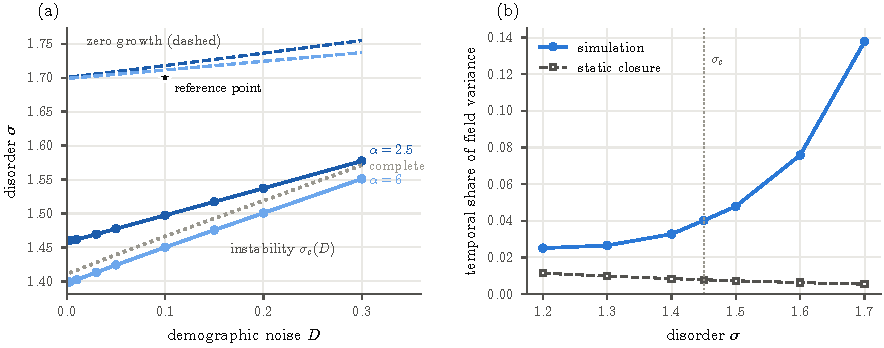
\includegraphics[width=0.8\linewidth]{figS_phase_lines.pdf}
\caption{(a) Instability line $\sigma_c(D)$ and zero-growth line from the static renewal theory at $\mu=-1.76$, for two degree tails and the complete graph; the star is the reference point.
(b) Share of the field variance that moves in time, simulation against the static closure ($\alpha=6$,
$D=0.1$, $N=4000$, $C=100$).  Source: \texttt{notebooks/02\_phase\_diagram.ipynb}.}
\label{fig:phaselines}
\end{figure}

\begin{table}[h]
\caption{Static renewal theory against simulation at $\alpha=6$, $D=0.1$, $N=4000$, $C=100$ (two economies
per $\sigma$; theory $\sigma_c=1.451$).  Source: \texttt{notebooks/02\_phase\_diagram.ipynb}.}
\label{tab:phase}
\begin{ruledtabular}
\begin{tabular}{cccc}
$\sigma$ & turnover (sim) & turnover (theory) & temporal share of field variance (sim)\\
\hline
1.20 & 0.309 & 0.307 & 0.025\\
1.30 & 0.368 & 0.368 & 0.027\\
1.40 & 0.435 & 0.435 & 0.033\\
1.45 & 0.470 & 0.471 & 0.040\\
1.50 & 0.511 & 0.509 & 0.048\\
1.60 & 0.598 & 0.588 & 0.076\\
1.70 & 0.688 & 0.673 & 0.138\\
\end{tabular}
\end{ruledtabular}
\end{table}

%======================================================================
\section{One-firm reduction, volatility law and multiscaling}
\label{sec:law}

\paragraph{Reduction.}  Table~\ref{tab:reduction} compares the full model with independent firms driven
by their measured fields and fresh noise, on the two reference economies.

\begin{figure}[h]
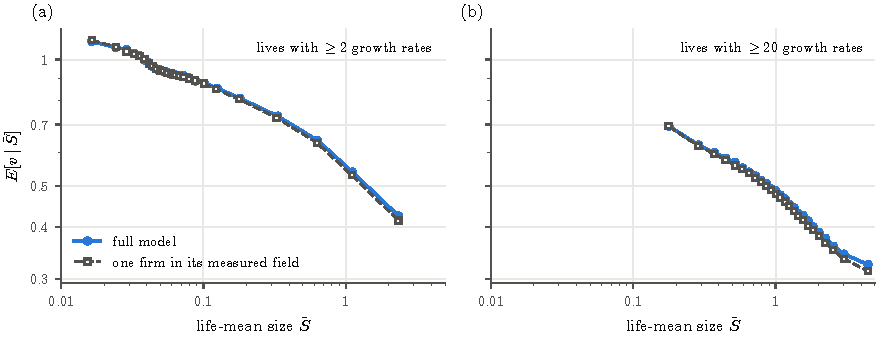
\includegraphics[width=0.75\linewidth]{figS_reduction.pdf}
\caption{One-firm reduction: life-panel volatility of the full model and of independent firms driven by
their measured fields and their own noise (two reference economies, $N=16000$).  Source:
\texttt{notebooks/04\_volatility\_law.ipynb}.}
\label{fig:reduction}
\end{figure}

\begin{table}[h]
\caption{Full model against one firm in its measured field: $\zeta_1$ and $\zeta_q/\zeta_1$ ($q=2,3,4$) of the
life panel.  Reference point, $N=16000$, two economies; exit rates $0.621$ (full) and $0.621$ (one
firm) per node per unit time.  Source: \texttt{notebooks/04\_volatility\_law.ipynb}.}
\label{tab:reduction}
\begin{ruledtabular}
\begin{tabular}{lcccc}
$n_{\min}$ & $\zeta_1$ full & $\zeta_1$ one firm & $\zeta_q/\zeta_1$ full & $\zeta_q/\zeta_1$ one firm\\
\hline
2  & 0.179 & 0.185 & 2.42, 3.97, 5.51 & 2.41, 3.97, 5.55\\
5  & 0.209 & 0.216 & 1.94, 2.74, 3.36 & 1.94, 2.76, 3.41\\
10 & 0.222 & 0.228 & 1.82, 2.42, 2.82 & 1.81, 2.42, 2.81\\
20 & 0.254 & 0.263 & 1.80, 2.42, 2.88 & 1.81, 2.44, 2.90\\
\end{tabular}
\end{ruledtabular}
\end{table}

\paragraph{Volatility law.}  Table~\ref{tab:law} gives the decomposition of Eq.~(8) of the main text by
deciles of life-mean size.  The prediction is within $5\%$ above the lowest decile and $9\%$ in it,
where the linearisation of the noise around the noise-free path is worst.  The fitness part is flat,
$\sqrt{V_F}=0.32$--$0.37$; the two parts are equal at $\Sb\simeq1.6$.  Over the range of the table the
measured slope of $\mathrm{sd}(g)$ against $\Sb$ is $0.17$ and the prediction's $0.22$.  The field used here
includes the entry dilution of Sec.~\ref{sec:relative}; without it the one-firm exit rate is $2\%$ low.

\begin{table}[h]
\caption{Volatility law, lives with at least $20$ growth rates of the two reference economies
($197\,636$ lives), by deciles of $\Sb$.  Source: \texttt{notebooks/04\_volatility\_law.ipynb}.}
\label{tab:law}
\begin{ruledtabular}
\begin{tabular}{cccccc}
$\Sb$ & sd$(g)$ & $\sqrt{V_F+B}$ & ratio & $\sqrt{V_F}$ & $\sqrt B$\\
\hline
0.26 & 0.726 & 0.793 & 1.09 & 0.323 & 0.724\\
0.46 & 0.668 & 0.683 & 1.02 & 0.353 & 0.585\\
0.64 & 0.636 & 0.639 & 1.01 & 0.364 & 0.526\\
0.81 & 0.613 & 0.604 & 0.98 & 0.367 & 0.479\\
0.99 & 0.589 & 0.578 & 0.98 & 0.370 & 0.445\\
1.19 & 0.568 & 0.551 & 0.97 & 0.368 & 0.411\\
1.43 & 0.547 & 0.529 & 0.97 & 0.366 & 0.381\\
1.73 & 0.525 & 0.506 & 0.96 & 0.365 & 0.350\\
2.20 & 0.500 & 0.479 & 0.96 & 0.364 & 0.312\\
3.53 & 0.478 & 0.456 & 0.95 & 0.374 & 0.260\\
\end{tabular}
\end{ruledtabular}
\end{table}

\paragraph{The identity with a composition term.}  Let $p(u\mid\Sb)$ be the law of the floor at fixed
size and $E_q(\Sb)=\int p(u\mid\Sb)\,(u+B(\Sb))^{q/2}\,du$, so that $\E[v^q\mid\Sb]=E_q\,\E[\epsilon^q]$.  Then
\begin{equation}
\zeta_q=-\frac{d\ln E_q}{d\ln\Sb}=\frac q2\,b\,\langle w\rangle_q-c_q,\qquad
c_q=\frac{1}{E_q}\int\frac{\partial p(u\mid\Sb)}{\partial\ln\Sb}\,(u+B)^{q/2}\,du ,
\label{eq:identity}
\end{equation}
with $b=-d\ln B/d\ln\Sb$ and $\langle w\rangle_q$ as in Eq.~(10).  The composition term $c_q$ vanishes if the
law of the floor does not depend on size.  On the network it does not vanish: larger lives have
larger degrees on average, and the floor grows with the degree, so $c_q>0$ and the decline is slower
than the noise share alone implies.  If the law of $\ln u$ only shifts with size, by $\delta(\Sb)$, then
$c_q=(q/2)(1-\langle w\rangle_q)\,d\delta/d\ln\Sb$ and $\zeta_q=(q/2)\,[\,b\langle w\rangle_q-(1-\langle w\rangle_q)\,d\delta/d\ln\Sb\,]$: a
rising floor flattens the decline and, since $\langle w\rangle_q$ falls with $q$, adds to the bend; a floor whose upper
tail spreads with size adds more.  If the floor is the same for all firms of a given size, $E_q=(u+B)^{q/2}$
and $\zeta_q=q\zeta_1$ exactly, whatever $c_q$: heterogeneity at fixed size is necessary for the bend in
general, and sufficient when $c_q=0$.  The tests in the main text use the measured floors of the lives in
each bin, which include the composition term.

\paragraph{Monotonicity of $\langle w\rangle_q$.}  With $Y=u+B$, $\langle w\rangle_q=B\,\E[Y^{q/2-1}]/\E[Y^{q/2}]=
B\exp[h(q-2)-h(q)]$, where $h(q)=\ln\E[Y^{q/2}]$ is the cumulant generating function of $\tfrac12\ln Y$
evaluated at $q$ and therefore convex.  Convexity makes $h(q)-h(q-2)$ non-decreasing, so $\langle w\rangle_q$ is
non-increasing in $q$, strictly unless $Y$ is degenerate at fixed size.

\paragraph{Per-life decomposition.}  Table~\ref{tab:mslaw} gives the exponents of the same lives under the
measured volatility and three laws built from the per-life decomposition, on both graphs, and
Table~\ref{tab:fifths} the quantities of the identity by fifths of size.  The per-life demographic part
$B$ is an estimate from the life's sizes; its dispersion within a size bin ($\Var\ln B=0.22$--$0.60$ by fifth on the
power-law graph) is larger than the measured volatilities allow, and with it the high-$q$ exponents
explode (rows ``own floor + own noise'').  The law with the bin mean of $B$ isolates the floor.

\begin{table}[h]
\caption{$\zeta_q$ ($q=1$--$4$) and $\zeta_q/\zeta_1$ of the lives with at least $20$ growth rates, volatility
as the growth standard deviation.  ``Own'' is the life's value, ``bin'' its mean in the life's size bin
($25$ equal-count bins).  Reference point, $N=16000$, two economies per graph.  Source:
\texttt{notebooks/05\_multiscaling.ipynb}.}
\label{tab:mslaw}
\begin{ruledtabular}
\begin{tabular}{llll}
graph & law & $\zeta_q$ & $\zeta_q/\zeta_1$\\
\hline
power law & measured $\Var g$ & 0.189, 0.335, 0.444, 0.525 & 1.77, 2.35, 2.78\\
 & own floor + bin noise & 0.232, 0.431, 0.593, 0.715 & 1.86, 2.56, 3.09\\
 & own floor + own noise & 0.233, 0.431, 0.682, 1.192 & 1.85, 2.92, 5.11\\
 & bin floor + own noise & 0.207, 0.431, 0.754, 1.361 & 2.08, 3.65, 6.58\\
regular & measured $\Var g$ & 0.395, 0.762, 1.097, 1.399 & 1.93, 2.78, 3.54\\
 & own floor + bin noise & 0.431, 0.856, 1.271, 1.674 & 1.98, 2.95, 3.88\\
 & own floor + own noise & 0.441, 0.856, 1.266, 1.725 & 1.94, 2.87, 3.92\\
 & bin floor + own noise & 0.430, 0.856, 1.295, 1.791 & 1.99, 3.01, 4.17\\
\end{tabular}
\end{ruledtabular}
\end{table}

\begin{table}[h]
\caption{The identity by fifths of size (power-law graph; regular graph in brackets).  $s^2$ is the
within-bin variance of $\ln(V_F+B)$ with $B$ at its bin mean, and the last two columns compare
$\langle w\rangle_4/\langle w\rangle_1$ with the lognormal estimate $e^{-3s^2/2}$.  Source: as Table~\ref{tab:mslaw}.}
\label{tab:fifths}
\begin{ruledtabular}
\begin{tabular}{cccccccc}
$\Sb$ & mean $\kappa$ & $\Var\ln V_F$ & share by degree & $b$ & $\langle w\rangle_1$ & $s^2$ & $\langle w\rangle_4/\langle w\rangle_1$ vs $e^{-3s^2/2}$\\
\hline
0.36 (0.29) & 0.76 & 0.51 (0.38) & 0.14 & 0.66 (0.73) & 0.79 (0.86) & 0.021 (0.008) & 0.96, 0.97 (0.99, 0.99)\\
0.72 (0.60) & 0.82 & 0.44 (0.29) & 0.20 & 0.76 (0.64) & 0.67 (0.78) & 0.048 (0.015) & 0.92, 0.93 (0.98, 0.98)\\
1.09 (0.91) & 0.89 & 0.50 (0.30) & 0.25 & 0.82 (0.87) & 0.60 (0.73) & 0.077 (0.022) & 0.86, 0.89 (0.96, 0.97)\\
1.58 (1.35) & 1.01 & 0.58 (0.33) & 0.31 & 0.87 (1.18) & 0.53 (0.71) & 0.121 (0.030) & 0.79, 0.83 (0.95, 0.96)\\
2.86 (2.55) & 1.51 & 0.85 (0.77) & 0.37 & 0.76 (1.97) & 0.43 (0.68) & 0.253 (0.053) & 0.62, 0.68 (0.89, 0.92)\\
\end{tabular}
\end{ruledtabular}
\end{table}

The local exponents of the law ``own floor + bin noise'' agree with $(q/2)\,b\,\langle w\rangle_q$ to about $10\%$
in the four lower fifths of the power-law graph; in the largest fifth the local exponents are smaller
($0.13$, $0.18$, $0.13$, $0.00$ against $0.16$, $0.29$, $0.37$, $0.41$), the effect of the composition term as
the mean degree rises from $1.01$ to $1.51$.

\paragraph{A fitted floor.}  An alternative test, without the noise-free integration, fits
$v^2=A\kappa^g+B_j$ (mean absolute deviation, one $B_j$ per size bin) to the same lives.  It gives
$g=1.00$ and predicts ratios $1.86$, $2.56$, $3.06$ against $1.80$, $2.42$, $2.88$ measured; the same law at
the mean degree gives exactly $2$, $3$, $4$ (\texttt{notebooks/05\_multiscaling.ipynb}).  The
fit assigns all of the top bins' variance to the floor ($B_j\to0$), so its partition differs from the
physical one of Table~\ref{tab:fifths}.

%======================================================================
\section{Robustness}
\label{sec:robust}

\paragraph{Production run and collective bursts.}  The facts of the main text come from eight economies
at the reference point with $N=32000$ (\texttt{notebooks/06\_facts.ipynb}).  In seven of them the aggregate
volatility per year is $0.03$--$0.23$ and $\zeta_1$ ($n_{\min}=5$) is $0.19$--$0.24$.  The eighth is in a
collective burst: its aggregate volatility is $0.54$, its turnover $0.68$ against $0.56$--$0.65$, and
volatility hardly depends on size ($\zeta_1=0.07$, ratios $1.54$, $1.56$, $1.15$).  We exclude economies
whose aggregate volatility exceeds $0.3$ (\texttt{kept} in \texttt{notebooks/06\_facts.ipynb}); with the burst included the pooled
exponents are $\zeta_q=0.167$, $0.297$, $0.378$, $0.411$ and the ratios $1.78$, $2.26$, $2.46$, because the burst
economy contributes the largest number of lives.  Across all $80$ economies of
Table~\ref{tab:robust}, $5$ exceed the threshold.  What triggers a burst is open.

\begin{table}[h]
\caption{Robustness of the life panel ($n_{\min}=5$, mean absolute deviation, all bins).  Economies: kept
over simulated, after the burst exclusion; $\zeta_1$ is pooled over the kept economies, $\pm$ its standard
deviation between economies; aggregate volatility per step and turnover per node per unit time are
means over economies; the aggregate growth here omits the entry term $D\nu$ of $\bar f$, which raises the aggregate
volatility by about $4\%$ and leaves the burst classification unchanged.  The $N$ sequence and the neighbourhood were run at $\sigma=1.75$, the point
before the retune.  Source: \texttt{notebooks/06\_facts.ipynb}.}
\label{tab:robust}
\begin{ruledtabular}
\begin{tabular}{lcccccccccc}
 & $\alpha$ & $\sigma$ & $D$ & $N$ & $C$ & economies & $\zeta_1$ & $\zeta_q/\zeta_1$ & agg.\ vol. & turnover\\
\hline
production & 2.5 & 1.70 & 0.10 & 32000 & 200 & 7/8 & $0.205\pm0.020$ & 1.92, 2.70, 3.31 & 0.081 & 0.597\\
\hline
$N$ sequence & 2.5 & 1.75 & 0.10 & 8000 & 200 & 8/8 & $0.188\pm0.039$ & 1.91, 2.67, 3.28 & 0.088 & 0.686\\
 & 2.5 & 1.75 & 0.10 & 16000 & 200 & 4/4 & $0.124\pm0.052$ & 1.82, 2.42, 2.80 & 0.108 & 0.693\\
 & 2.5 & 1.75 & 0.10 & 32000 & 200 & 5/6 & $0.123\pm0.030$ & 1.83, 2.42, 2.78 & 0.112 & 0.678\\
 & 2.5 & 1.75 & 0.10 & 64000 & 200 & 2/2 & $0.143\pm0.003$ & 1.88, 2.57, 3.06 & 0.071 & 0.635\\
\hline
neighbourhood & 2.5 & 1.75 & 0.05 & 8000 & 200 & 4/4 & $0.152\pm0.030$ & 1.84, 2.47, 2.89 & 0.106 & 0.620\\
 & 2.5 & 1.75 & 0.20 & 8000 & 200 & 4/4 & $0.250\pm0.035$ & 1.97, 2.84, 3.58 & 0.097 & 0.769\\
 & 2.5 & 1.70 & 0.10 & 8000 & 200 & 3/4 & $0.257\pm0.036$ & 1.97, 2.86, 3.64 & 0.039 & 0.533\\
 & 2.5 & 1.80 & 0.10 & 8000 & 200 & 3/4 & $0.107\pm0.074$ & 1.79, 2.36, 2.73 & 0.147 & 1.049\\
 & 3 & 1.75 & 0.10 & 8000 & 200 & 4/4 & $0.190\pm0.041$ & 1.95, 2.81, 3.56 & 0.087 & 0.709\\
 & 2.5 & 1.75 & 0.10 & 8000 & 100 & 3/4 & $0.157\pm0.066$ & 1.76, 2.26, 2.55 & 0.158 & 1.108\\
 & 2.5 & 1.75 & 0.10 & 8000 & 400 & 4/4 & $0.170\pm0.038$ & 1.93, 2.75, 3.46 & 0.069 & 0.642\\
\hline
retune & 2.5 & 1.70 & 0.10 & 16000 & 200 & 4/4 & $0.198\pm0.018$ & 1.93, 2.71, 3.32 & 0.080 & 0.596\\
 & 2.5 & 1.70 & 0.15 & 16000 & 200 & 4/4 & $0.232\pm0.020$ & 1.98, 2.88, 3.66 & 0.060 & 0.585\\
 & 2.5 & 1.70 & 0.20 & 16000 & 200 & 4/4 & $0.251\pm0.018$ & 2.00, 2.94, 3.79 & 0.056 & 0.583\\
 & 2.5 & 1.72 & 0.10 & 16000 & 200 & 4/4 & $0.171\pm0.024$ & 1.88, 2.56, 3.05 & 0.111 & 0.620\\
 & 2.5 & 1.72 & 0.15 & 16000 & 200 & 4/4 & $0.202\pm0.024$ & 1.93, 2.72, 3.33 & 0.094 & 0.615\\
 & 2.5 & 1.72 & 0.20 & 16000 & 200 & 4/4 & $0.238\pm0.012$ & 1.99, 2.91, 3.70 & 0.070 & 0.602\\
\end{tabular}
\end{ruledtabular}
\end{table}

Table~\ref{tab:robust} collects all runs.

At $\sigma=1.75$ (the point before retuning), $\zeta_1$ for $n_{\min}=5$ is $0.188$, $0.124$, $0.123$, $0.143$ at
$N=8000$, $16000$, $32000$, $64000$, and the ratio curve $1.91$, $1.82$, $1.83$, $1.88$ for $q=2$: the
exponent converges by $N\simeq16000$ within the spread between economies ($\pm0.03$), and the shape of
the curve and the ratios do not depend on $N$.  At $N=8000$ the configuration graph with $\alpha=2.5$ and
$C=200$ is saturated: merging multi-edges removes $40\%$ of the edge ends.  At $N=16000$ the retune over
$\sigma\in\{1.70,1.72\}$ and $D\in\{0.1,0.15,0.2\}$ gives $\zeta_1=0.17$--$0.25$ ($n_{\min}=5$), with $\zeta_1$ growing
with $D$ and falling with $\sigma$; the reference point $\sigma=1.70$, $D=0.1$ gives $\zeta_q=0.198$, $0.382$, $0.537$,
$0.657$.

\paragraph{Softer and harder self-limitation.}  Table~\ref{tab:theta} replaces the self-limitation and
the interactions by $(x_i/m)^\theta$ and $\sum_jJ_{ij}(x_j/m)^\theta$ (main text, Sec.~VIII) at $\alpha=2.5$, $D=0.1$, $C=200$,
$N=16000$, four economies per row, none in a burst.  The temporal share of the field variance is measured on
one economy with $N=8000$ over a window of $100$.

\begin{table}[h]
\caption{Self-limitation exponent $\theta$ with noise ($n_{\min}=5$).  $R$: decades spanned by the $25$ bins;
$\pm$: standard deviation of $\zeta_1R$ between economies; volatility of the smallest and largest bin;
Hill index of the top $1\%$ of sizes.  The $\theta=1$ row is the retune economy at the reference point.
Source: \texttt{notebooks/06\_facts.ipynb}.}
\label{tab:theta}
\begin{ruledtabular}
\begin{tabular}{ccccccccc}
$\theta$ & $\sigma$ & $\zeta_1$ & $R$ & $\zeta_1R$ & $\zeta_q/\zeta_1$ & volatility & size Hill & temporal share\\
\hline
1.5 & 1.70 & 0.105 & 1.89 & $0.20\pm0.04$ & 1.75, 2.21, 2.41 & 1.12, 0.62 & 6.7 & 0.204\\
1 & 1.70 & 0.198 & 2.00 & $0.40\pm0.04$ & 1.93, 2.71, 3.32 & 1.11, 0.41 & 4.6 & 0.165\\
0.75 & 1.70 & 0.289 & 1.98 & $0.57\pm0.03$ & 2.03, 3.05, 4.05 & 1.11, 0.30 & 3.8 & 0.125\\
0.5 & 1.70 & 0.338 & 1.71 & $0.58\pm0.01$ & 2.08, 3.24, 4.45 & 1.11, 0.29 & 2.7 & 0.018\\
0.5 & 1.90 & 0.266 & 2.13 & $0.57\pm0.03$ & 2.05, 3.12, 4.18 & 1.12, 0.33 & 2.2 & 0.176\\
0.5 & 2.00 & 0.186 & 2.35 & $0.44\pm0.01$ & 2.02, 3.01, 3.94 & 1.12, 0.45 & 2.0 & 0.262\\
\end{tabular}
\end{ruledtabular}
\end{table}

%======================================================================
\section{Protocol}
\label{sec:protocol}

\paragraph{The year.}  We sample every $0.5$ time units.  The lag-one autocorrelation of growth within
lives is $+0.13$, $+0.18$ and $0.00$ at steps $0.5$, $1$ and $2$; a step of $2$ would remove it but leaves
too few growth rates per life for the panel.  In the two reference economies, lives with at least five
growth rates give $\zeta_q=0.209$, $0.405$, $0.572$, $0.702$ (ratios $1.94$, $2.74$, $3.36$) over $2.0$
decades at step $0.5$, and $\zeta_q=0.156$, $0.270$, $0.339$, $0.370$ (ratios $1.73$, $2.17$, $2.36$) over
$1.4$ decades at step $2$: volatility per step rises by a factor $1.1$ in the smallest size bin and $2.2$
in the largest, so the decline flattens, and the ratio curve bends further below $q$.  For lives with
at least $20$ growth rates the change is smaller ($\zeta_1=0.254$ and $0.230$, ratios $1.80$, $2.42$,
$2.88$ and $1.75$, $2.27$, $2.60$, although at step $2$ these lives span only $0.9$ decades).  The bend
below $q$ survives the coarser year; the level of $\zeta_1$ for short lives does not
(\texttt{notebooks/06\_facts.ipynb}).

\paragraph{Minimum life length.}  MSB keep every firm with at least two growth rates; their firms have $46$ on
average, and their results do not change for firms with at least $20$.  The model's lives are much shorter:
$38\%$ of the lives with at least two growth rates have exactly two ($N=16000$).  The main text therefore uses
$n_{\min}=20$ for the facts, as for the theory tests.  In the production run $\zeta_q=0.178$, $0.431$, $0.706$, $0.968$
(ratios $2.42$, $3.96$, $5.43$) for $n_{\min}=2$, $0.205$, $0.394$, $0.554$, $0.679$ ($1.92$, $2.70$, $3.31$) for $n_{\min}=5$,
$0.214$, $0.381$, $0.501$, $0.577$ ($1.79$, $2.35$, $2.70$) for $n_{\min}=10$ and $0.249$, $0.443$, $0.587$, $0.688$ ($1.78$, $2.35$,
$2.76$) for $n_{\min}=20$, over $2.1$, $2.0$, $1.8$ and $1.4$ decades: the ratios lie above $q$ for $n_{\min}=2$ and below
from $n_{\min}=5$, and the range shrinks because long lives do not occur at the newborn sizes.

\paragraph{The tail index $b$.}  For lives with at least two growth rates the model gives
$b=4.40$--$4.44$ at every parameter point, close to the Compustat value $4.6$.  A null with iid Laplace
growth rates, no differences between firms and the model's distribution of life lengths gives
$4.34$, so the agreement is an effect of short lives.  For longer lives $b$ grows: $5.5$ and $6.8$ in the production
run for $n_{\min}=10$ and $20$ ($5.7$ and $6.9$ at $N=16000$), against $9.3$ and $12.6$ for the Laplace null and $4.6$ in
Compustat for both samples (\texttt{notebooks/06\_facts.ipynb}).

\paragraph{Volatility estimator.}  With the standard deviation instead of $\sqrt{\pi/2}$ times the mean
absolute deviation, $\zeta_1$ is $0.03$ lower and the ratios are $0.03$--$0.3$ higher (\texttt{notebooks/06\_facts.ipynb},
rows SD; production run: $\zeta_1=0.175$, ratios $1.96$, $2.82$, $3.58$ at $n_{\min}=5$).

\bibliography{bib}

\end{document}
